\subsubsection{Normalization}

Since not all voices will be recorded at exactly the same level, it is important to normalize
the amplitude of each sample in order to ensure that features will be comparable.  Audio
normalization is analogous to image normalization.  Since all samples are to be loaded as
floating point values in the range $[-1.0, 1.0]$, it should be ensured that every sample actually
does cover this entire range.

The procedure is relatively simple: find the maximum amplitude in the sample, and then scale
the sample by dividing each point by this maximum. Figure \ref{fig:prep-norm} illustrates
normalized input wave signal.

\begin{figure}
	\centering
	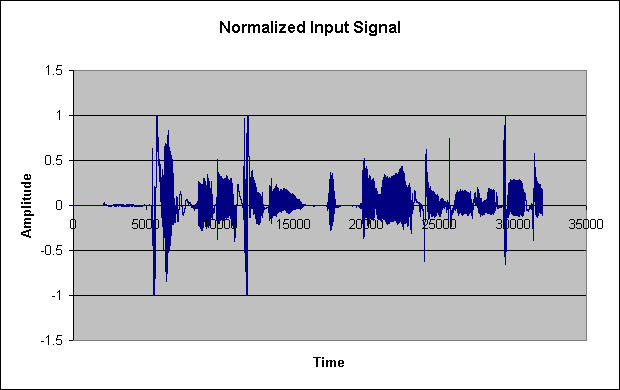
\includegraphics[width=400pt]{../graphics/graphs/wav-normalized.png}
	\caption{Normalization of aihua5.wav from the testing set.}
	\label{fig:prep-norm}
\end{figure}
